\subsection{Image moments}

Thanks the preprocessing done by FPGA, the \locate* task is equivalent to finding homogeneous regions of white pixels on top of a black background.
This task is implemented by the function \texttt{FindContours}~\cite{findcontours} from \texttt{OpenCV}, that finds a rectangular bounding box around pixels with the same intensity.
The precise coordinates of the bubble centroid can be found by computing the centroid (the image moments, see section~\ref{sec:backgr:moments}) of each bounding box.

\subsubsection{Algorithm}

\begin{enumerate}
	\itemsep 0em
	\item Through \texttt{OpenCV}'s \texttt{FindContours}, find all the bubbles for a given frame;
	\item For each region in the output:
	      \begin{enumerate}
		      \item Compute the image moments with \texttt{OpenCV}'s \texttt{moments} function;
		      \item Use the moments of order 0 and 1 to compute the centroids;
		      \item Add the coordinates to the output list.
	      \end{enumerate}
\end{enumerate}

\subsubsection{Evaluation}

As visible in figure~\ref{fig:locate:moments}, the result quality is almost perfect, finding about 99\% of bubbles.
The speed of 67 FPS is extremely good as well, while still being lower than the target.

\begin{figure}
	\centerline{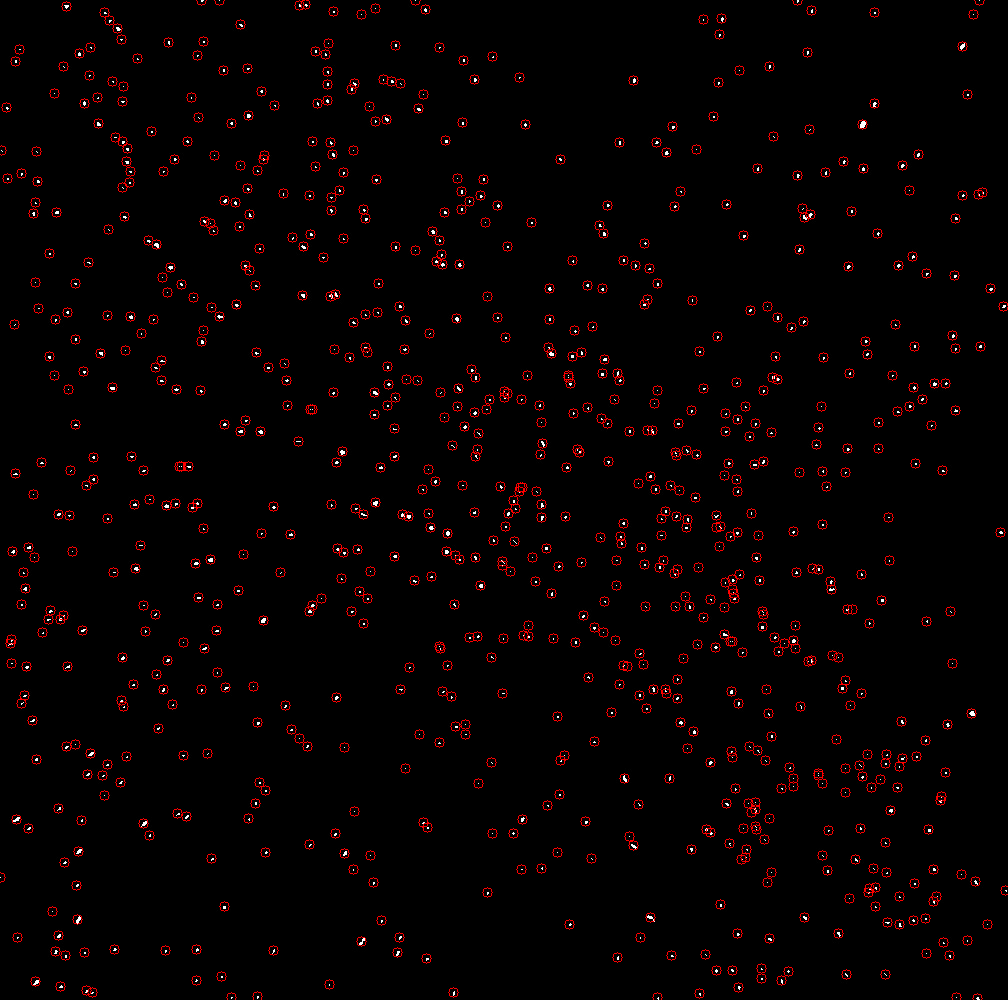
\includegraphics[width=\locateimgsize]{images/locate/opencv moments.png}}
	\caption{\centering Image moments's result}
	\label{fig:locate:moments}
\end{figure}
